\documentclass[11pt]{article}
\usepackage{amsmath}
\usepackage{amssymb}
\usepackage{graphicx}
\usepackage{tabularx}
\usepackage{fancyhdr}
\usepackage{lastpage}

% Page layout
\usepackage[top=1in, bottom=1in, left=1in, right=1in]{geometry}

% Header and footer
\pagestyle{fancy}
\fancyhf{}
\rfoot{Page \thepage}
\renewcommand{\headrulewidth}{0pt}

% Modified Question command with left-aligned number
\newcommand{\questiona}[2]{
    \noindent\textbf{Q#2.} #1 \hfill \textbf{[1 Mark]}
}

\newcommand{\questionb}[2]{
    \noindent\textbf{Q#2.} #1 \hfill \textbf{[2 Marks]}
}

\begin{document}

% Title section with horizontal line
\begin{center}
    \Large\textbf{GATE 2017 - Instrumentation Engineering (IN)} \\
    \large\textbf{General Aptitude and Technical Questions} \\
    \rule{\textwidth}{0.5pt} % Horizontal line below heading
\end{center}

\vspace{0.5cm}

% General Aptitude Section
\section*{General Aptitude}

\questiona{The event would have been successful if you \_\_\_\_\_ able to come.}{1}
\begin{enumerate}
    \item[(A)] are  
    \item[(B)] had been  
    \item[(C)] have been  
    \item[(D)] would have been  
\end{enumerate}
\vspace{0.5cm}

\questiona{There was no doubt that their work was thorough.

Which of the words below is closest in meaning to the underlined word above?}{2}
\begin{enumerate}
    \item[(A)] pretty  
    \item[(B)] complete  
    \item[(C)] sloppy  
    \item[(D)] haphazard  
\end{enumerate}
\vspace{0.5cm}

\questiona{Four cards lie on a table. Each card has a number printed on one side and a colour on the other. The faces visible on the cards are 2, 3, red, and blue.

Proposition: If a card has an even value on one side, then its opposite face is red.

The cards which MUST be turned over to verify the above proposition are}{3}
\begin{enumerate}
    \item[(A)] 2, red  
    \item[(B)] 2, 3, red  
    \item[(C)] 2, blue  
    \item[(D)] 2, red, blue  
\end{enumerate}
\vspace{0.5cm}

\questiona{What is the value of \( x \) when \( 81 \times \left( \frac{16}{25} \right)^{x+2} + \left( \frac{3}{5} \right)^{2x+4} = 144 \)?}{4}
\begin{enumerate}
    \item[(A)] 1  
    \item[(B)] -1  
    \item[(C)] -2  
    \item[(D)] Cannot be determined  
\end{enumerate}
\vspace{0.5cm}

\questiona{Two dice are thrown simultaneously. The probability that the product of the numbers appearing on the top faces of the dice is a perfect square is}{5}
\begin{enumerate}
    \item[(A)] 1/9  
    \item[(B)] 2/9  
    \item[(C)] 1/3  
    \item[(D)] 4/9  
\end{enumerate}
\vspace{0.5cm}

\questionb{Bhaichung was observing the pattern of people entering and leaving a car service centre. There was a single window where customers were being served. He saw that people inevitably came out of the centre in the order that they went in. However, the time they spent inside seemed to vary a lot: some people came out in a matter of minutes while for others it took much longer.

From this, what can one conclude?}{6}
\begin{enumerate}
    \item[(A)] The centre operates on a first-come-first-served basis, but with variable service times, depending on specific customer needs.  
    \item[(B)] Customers were served in an arbitrary order, since they took varying amounts of time for service completion in the centre.  
    \item[(C)] Since some people came out within a few minutes of entering the centre, the system is likely to operate on a last-come-first-served basis.  
    \item[(D)] Entering the centre early ensured that one would have shorter service times and most people attempted to do this.  
\end{enumerate}
\vspace{0.5cm}

\questionb{A map shows the elevations of Darjeeling, Gangtok, Kalimpong, Pelling, and Siliguri.  
Kalimpong is at a lower elevation than Gangtok. Pelling is at a lower elevation than Gangtok.  
Pelling is at a higher elevation than Siliguri. Darjeeling is at a higher elevation than Gangtok.

Which of the following statements can be inferred from the paragraph above?

i. Pelling is at a higher elevation than Kalimpong  
ii. Kalimpong is at a lower elevation than Darjeeling  
iii. Kalimpong is at a higher elevation than Siliguri  
iv. Siliguri is at a lower elevation than Gangtok}{7}
\begin{enumerate}
    \item[(A)] Only ii    
    \item[(B)] Only ii and iii    
    \item[(C)] Only ii and iv    
    \item[(D)] Only iii and iv  
\end{enumerate}
\vspace{0.5cm}

\questionb{P, Q, R, S, T and U are seated around a circular table, R is seated two places to the right of Q. P is seated three places to the left of R. S is seated opposite U. If P and U now switch seats, which of the following must necessarily be true?}{8}
\begin{enumerate}
    \item[(A)] P is immediately to the right of R  
    \item[(B)] T is immediately to the left of P  
    \item[(C)] T is immediately to the left of P or P is immediately to the right of Q  
    \item[(D)] U is immediately to the right of R or P is immediately to the left of T  
\end{enumerate}
\vspace{0.5cm}

\questionb{Budhan covers a distance of 19 km in 2 hours by cycling one fourth of the time and walking the rest. The next day he cycles (at the same speed as before) for half the time and walks the rest (at the same speed as before) and covers 26 km in 2 hours. The speed in km/h at which Budhan walks is}{9}
\begin{enumerate}
    \item[(A)] 1    
    \item[(B)] 4    
    \item[(C)] 5    
    \item[(D)] 6
\end{enumerate}
\vspace{0.5cm}

\questionb{The points in the graph below represent the halts of a lift for durations of 1 minute, over a period of 1 hour.}{10}
\begin{center}
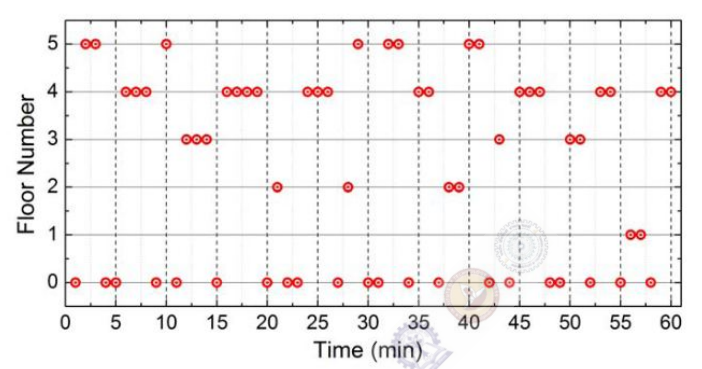
\includegraphics[width=0.5\textwidth]{figures/10.png}
\end{center}
Which of the following statements are correct?

i. The elevator never moves directly from any non-ground floor to another non-ground floor over the one hour period  
ii. The elevator stays on the fourth floor for the longest duration over the one hour period  
\begin{enumerate}
    \item[(A)] Only i    
    \item[(B)] Only ii    
    \item[(C)] Both i and ii    
    \item[(D)] Neither i nor ii
\end{enumerate}
\vspace{0.5cm}

% Technical Section
\section*{Technical Section}

\questiona{If \( v \) is a non-zero vector of dimension \( 3 \times 1 \), then the matrix  
\[ A = vv^T \]  
has a rank = \_\_\_\_\_.}{1}
\vspace{0.5cm}

\questiona{The figure shows a shape ABC and its mirror image \( A_1B_1C_1 \) across the horizontal axis (X-axis). The coordinate transformation matrix that maps ABC to \( A_1B_1C_1 \) is}{2}
\begin{center}
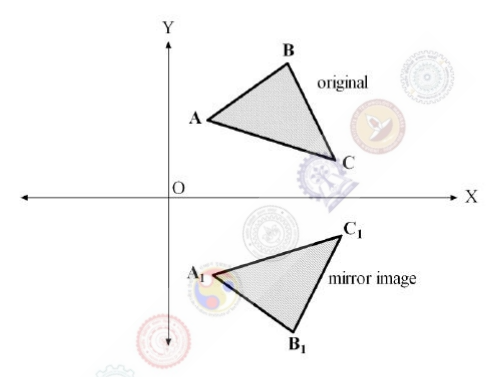
\includegraphics[width=0.5\textwidth]{figures/2.png}
\end{center}
\begin{enumerate}
    \item[(A)] \(\begin{bmatrix} 0 & 1 \\ 1 & 0 \end{bmatrix}\)
    \item[(B)] \(\begin{bmatrix} 0 & 1 \\ -1 & 0 \end{bmatrix}\)
    \item[(C)] \(\begin{bmatrix} -1 & 0 \\ 0 & 1 \end{bmatrix}\)
    \item[(D)] \(\begin{bmatrix} 1 & 0 \\ 0 & -1 \end{bmatrix}\)
\end{enumerate}
\vspace{0.5cm}

\questiona{Let \( z = x + jy \) where \( j = \sqrt{-1} \). Then \(\cos z =\)}{3}
\begin{enumerate}
    \item[(A)] \(\cos z\)  
    \item[(B)] \(\cos \overline{z}\)  
    \item[(C)] \(\sin z\)  
    \item[(D)] \(\sin \overline{z}\)
\end{enumerate}
\vspace{0.5cm}

\questiona{The eigenvalues of the matrix \( A = \begin{bmatrix} 1 & -1 & 5 \\ 0 & 5 & 6 \\ 0 & -6 & 5 \end{bmatrix} \) are}{4}
\begin{enumerate}
    \item[(A)] \(-1, 5, 6\)  
    \item[(B)] \(1, -5 \pm j6\)  
    \item[(C)] \(1, 5 \pm j6\)  
    \item[(D)] \(1, 5, 5\)
\end{enumerate}
\vspace{0.5cm}

\questiona{For a first order lowpass filter with unity d.c. gain and \(-3 \, \text{dB}\) corner frequency of \(2000\pi \, \text{rad/s}\), the transfer function \(H(j\omega)\) is}{5}
\begin{enumerate}
    \item[(A)] \(\frac{1}{1000 + j\omega}\)  
    \item[(B)] \(\frac{1}{1 + j1000\omega}\)  
    \item[(C)] \(\frac{2000\pi}{2000\pi + j\omega}\)  
    \item[(D)] \(\frac{1000\omega}{1 + j1000\omega}\)
\end{enumerate}
\vspace{0.5cm}

\questiona{A series R-L-C circuit is excited with a 50 V, 50 Hz sinusoidal source. The voltages across the resistance and the capacitance are shown in the figure. The voltage across the inductor (V_L) is \_\_\_\_\_ V.}{6}
\begin{center}
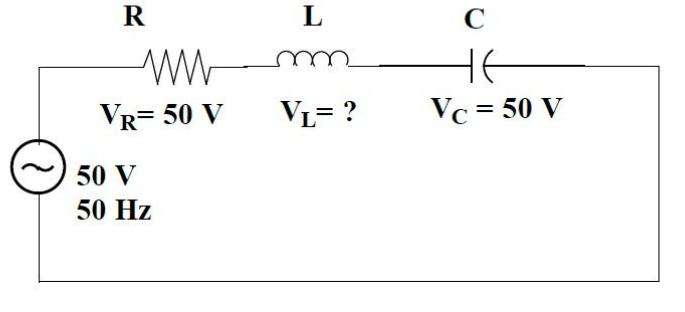
\includegraphics[width=0.5\textwidth]{figures/6.png}
\end{center}
\vspace{0.5cm}

\questiona{The connection of two 2-port networks is shown in the figure. The ABCD parameters of \( N1 \) and \( N2 \) networks are given as}{7}
\begin{center}
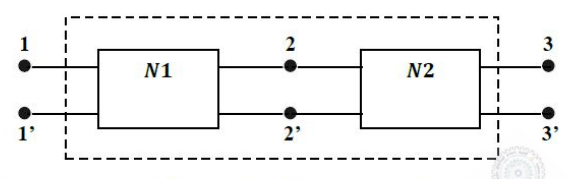
\includegraphics[width=0.5\textwidth]{figures/7.png}
\end{center}
\[
\begin{bmatrix} A & B \\ C & D \end{bmatrix}_{N1} = \begin{bmatrix} 1 & 5 \\ 0 & 1 \end{bmatrix}
\text{ and }
\begin{bmatrix} A & B \\ C & D \end{bmatrix}_{N2} = \begin{bmatrix} 1 & 0 \\ 0.2 & 1 \end{bmatrix}
\]
The ABCD parameters of the combined 2-port network are
\begin{enumerate}
    \item[(A)] \(\begin{bmatrix} 2 & 5 \\ 0.2 & 1 \end{bmatrix}\)
    \item[(B)] \(\begin{bmatrix} 1 & 2 \\ 0.5 & 1 \end{bmatrix}\)
    \item[(C)] \(\begin{bmatrix} 5 & 2 \\ 0.5 & 1 \end{bmatrix}\)
    \item[(D)] \(\begin{bmatrix} 1 & 2 \\ 0.5 & 5 \end{bmatrix}\)
\end{enumerate}
\vspace{0.5cm}

\questiona{A circuit consisting of dependent and independent sources is shown in the figure. If the voltage at Node-1 is \(-1 \, V\), then the voltage at Node-2 is \_\_\_\_\_ V.}{8}
\begin{center}
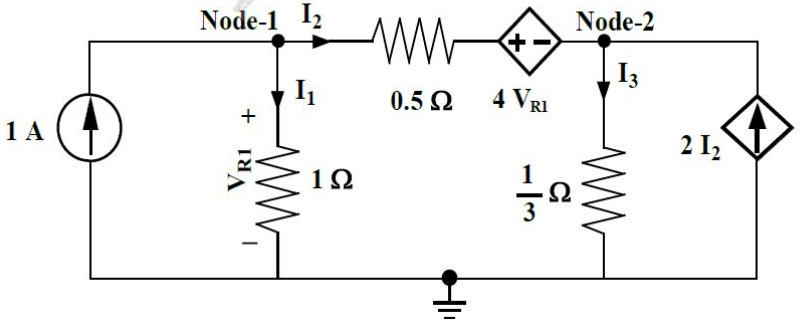
\includegraphics[width=0.5\textwidth]{figures/8.png}
\end{center}
\vspace{0.5cm}

\questiona{A periodic signal \( x(t) \) is shown in the figure. The fundamental frequency of the signal \( x(t) \) in Hz is \_\_\_\_\_.}{9}
\begin{center}
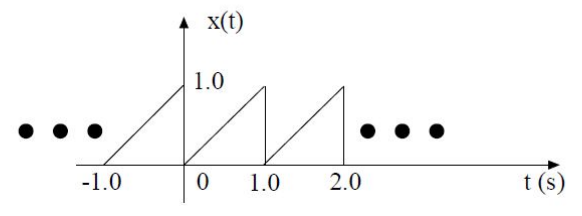
\includegraphics[width=0.5\textwidth]{figures/9.png}
\end{center}
\vspace{0.5cm}

\questiona{A system is described by the following differential equation:
\[\frac{dy(t)}{dt} + 2y(t) = \frac{dx(t)}{dt} + x(t), \quad x(0) = y(0) = 0\]
where \( x(t) \) and \( y(t) \) are the input and output variables respectively. The transfer function of the inverse system is}{10}
\begin{enumerate}
    \item[(A)] \(\frac{s+1}{s-2}\)  
    \item[(B)] \(\frac{s+2}{s+1}\)  
    \item[(C)] \(\frac{s+1}{s+2}\)  
    \item[(D)] \(\frac{s-1}{s-2}\)
\end{enumerate}
\vspace{0.5cm}

\questiona{If a continuous-time signal \( x(t) = \cos(2\pi t) \) is sampled at 4 Hz, the value of the discrete-time sequence \( x(n) \) at \( n = 5 \) is}{11}
\begin{enumerate}
    \item[(A)] -0.707  
    \item[(B)] -1  
    \item[(C)] 0  
    \item[(D)] 1  
\end{enumerate}
\vspace{0.5cm}

\questiona{The Region of Convergence (ROC) of the Z-transform of a causal unit step discrete-time sequence is}{12}
\begin{enumerate}
    \item[(A)] \(|z| < 1\)  
    \item[(B)] \(|z| \leq 1\)  
    \item[(C)] \(|z| > 1\)  
    \item[(D)] \(|z| \geq 1\)
\end{enumerate}
\vspace{0.5cm}

\questiona{The term hysteresis is associated with}{13}
\begin{enumerate}
    \item[(A)] ON-OFF control  
    \item[(B)] P-I control  
    \item[(C)] Feed-forward control  
    \item[(D)] Ratio control  
\end{enumerate}
\vspace{0.5cm}

\questiona{The differential amplifier, shown in the figure, has a differential gain of \( A_d = 100 \) and common mode gain of \( A_c = 0.1 \). If \( V_1 = 5.01 \, \text{V} \) and \( V_2 = 5.00 \, \text{V} \), then \( \text{Vo} \), in \textbf{volt} (up to one decimal place) is \_\_\_\_\_.}{14}
\begin{center}
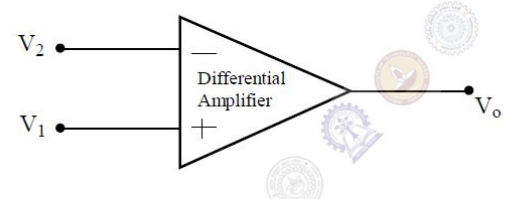
\includegraphics[width=0.5\textwidth]{figures/14.png}
\end{center}
\vspace{0.5cm}

\questiona{The silicon diode, shown in the figure, has a barrier potential of 0.7 V. There will be no forward current flow through the diode, if \( \text{V}_{dc} \), in \textbf{volt}, is greater than \_\_\_\_\_.}{15}
\begin{center}
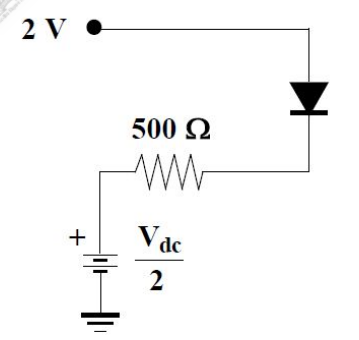
\includegraphics[width=0.5\textwidth]{figures/15.png}
\end{center}
\begin{enumerate}
    \item[(A)] 0.7  
    \item[(B)] 1.3  
    \item[(C)] 1.8  
    \item[(D)] 2.6  
\end{enumerate}
\vspace{0.5cm}

\questiona{The figure shows a phase locked loop. The output frequency is locked at \( f_0 = 5 \, \text{kHz} \). The value of \( f_i \) in kHz is \_\_\_\_\_.}{16}
\begin{center}
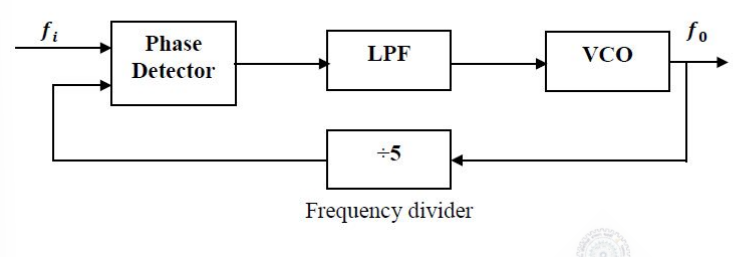
\includegraphics[width=0.5\textwidth]{figures/16.png}
\end{center}
\vspace{0.5cm}

\questiona{The condition for oscillation in a feedback oscillator circuit is that at the frequency of oscillation, initially the loop gain is greater than unity while the total phase shift around the loop in degree is}{17}
\begin{enumerate}
    \item[(A)] 0  
    \item[(B)] 90  
    \item[(C)] 180  
    \item[(D)] 270
\end{enumerate}
\vspace{0.5cm}

\questiona{The output \( V_O \) shown in the figure, in \textbf{volt}, is close to}{18}
\begin{center}
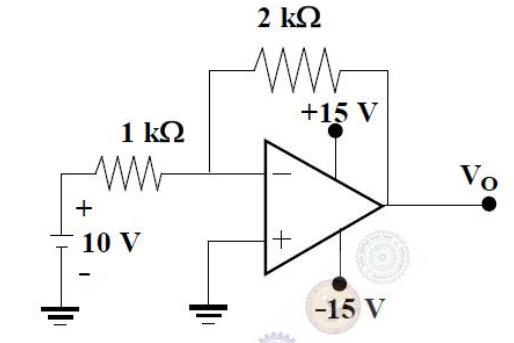
\includegraphics[width=0.5\textwidth]{figures/18.png}
\end{center}
\begin{enumerate}
    \item[(A)] -20  
    \item[(B)] -15  
    \item[(C)] -5  
    \item[(D)] 0  
\end{enumerate}
\vspace{0.5cm}

\questiona{An 8-bit microcontroller with 16 address lines has 3 fixed interrupts i.e., Int1, Int2 and Int3 with corresponding interrupt vector addresses as 0008H, 0010H and 0018H. To execute a 32-byte long Interrupt Service Subroutine for Int1 starting at the address ISS1, the location 0008H onwards should ideally contain}{19}
\begin{enumerate}
    \item[(A)] a CALL to ISS1  
    \item[(B)] an unconditional JUMP to ISS1  
    \item[(C)] a conditional JUMP to ISS1  
    \item[(D)] only ISS1  
\end{enumerate}
\vspace{0.5cm}

\questiona{A and B are the logical inputs and X is the logical output shown in the figure. The output X is related to A and B by}{20}
\begin{center}
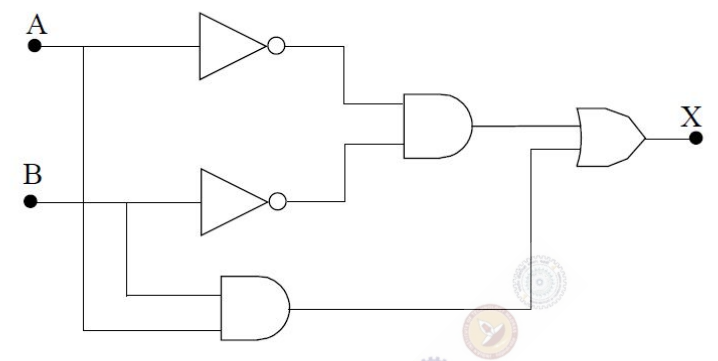
\includegraphics[width=0.5\textwidth]{figures/20.png}
\end{center}
\begin{enumerate}
    \item[(A)] \( X = \overline{AB} + \overline{BA} \)  
    \item[(B)] \( X = AB + \overline{BA} \)  
    \item[(C)] \( X = AB + \overline{AB} \)  
    \item[(D)] \( X = \overline{AB} + \overline{BA} \)  
\end{enumerate}
\vspace{0.5cm}

\questiona{A current waveform, i(t), shown in the figure, is passed through a Permanent Magnet Moving Coil (PMMC) type ammeter. The reading of the ammeter up to two decimal places is}{21}
\begin{center}
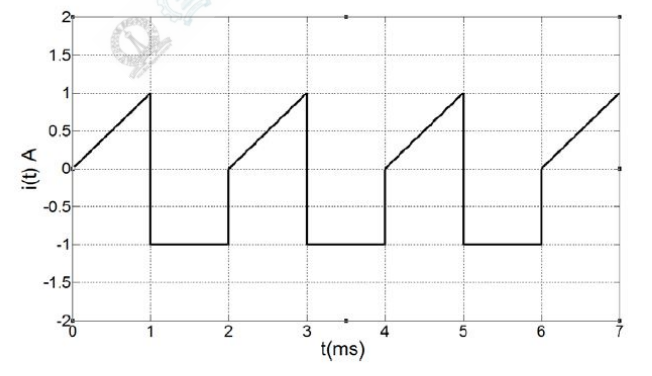
\includegraphics[width=0.5\textwidth]{figures/21.png}
\end{center}
\begin{enumerate}
    \item[(A)] -0.25 A  
    \item[(B)] -0.12 A  
    \item[(C)] 0.37 A  
    \item[(D)] 0.5 A  
\end{enumerate}
\vspace{0.5cm}

\questiona{Identify the instrument that does not exist:}{22}
\begin{enumerate}
    \item[(A)] Dynamometer-type ammeter  
    \item[(B)] Dynamometer-type wattmeter  
    \item[(C)] Moving-iron voltmeter  
    \item[(D)] Moving-iron wattmeter  
\end{enumerate}
\vspace{0.5cm}

\questiona{The most suitable pressure gauge to measure pressure in the range of \(10^{-4}\) to \(10^{-3}\) \textbf{torr} is}{23}
\begin{enumerate}
    \item[(A)] Bellows  
    \item[(B)] Barometer  
    \item[(C)] Strain gauge  
    \item[(D)] Pirani gauge  
\end{enumerate}
\vspace{0.5cm}

\questiona{The standard for long distance analog signal transmission in process control industry is}{24}
\begin{enumerate}
    \item[(A)] \(4 - 20 \, \text{mV}\)  
    \item[(B)] \(0 - 20 \, \text{mA}\)  
    \item[(C)] \(4 - 20 \, \text{mA}\)  
    \item[(D)] \(0 - 5 \, \text{V}\)  
\end{enumerate}
\vspace{0.5cm}

\questiona{The pressure drop across an orifice plate for a particular flow rate is \(5 \, \text{kg/m}^2\). If the flow rate is doubled (within the operating range of the orifice), the corresponding pressure drop in \(\text{kg/m}^2\) is}{25}
\begin{enumerate}
    \item[(A)] 2.5  
    \item[(B)] 5.0  
    \item[(C)] 20.0  
    \item[(D)] 25.0  
\end{enumerate}
\vspace{0.5cm}

\questionb{The probability that a communication system will have high fidelity is 0.81. The probability that the system will have both high fidelity and high selectivity is 0.18. The probability that a given system with high fidelity will have high selectivity is}{26}
\begin{enumerate}
    \item[(A)] 0.181  
    \item[(B)] 0.191  
    \item[(C)] 0.222  
    \item[(D)] 0.826  
\end{enumerate}
\vspace{0.5cm}

\questionb{The angle between two vectors \( x_1 = [2 \quad 6 \quad 14]^T \) and \( x_2 = [-12 \quad 8 \quad 16]^T \) in radian is \_\_\_\_\_.}{27}
\vspace{0.5cm}

\questionb{The following table lists an \( n^{\text{th}} \) order polynomial \( f(x) = a_nx^n + a_{n-1}x^{n-1} + \cdots + a_1x + a_0 \) and the forward differences evaluated at equally spaced values of \( x \). The order of the polynomial is}{28}
\begin{center}
\begin{tabular}{|c|c|c|c|c|}
\hline
\( x \) & \( f(x) \) & \( \Delta f \) & \( \Delta^2 f \) & \( \Delta^3 f \) \\ \hline
-0.4 & 1.7648 & -0.2965 & 0.089 & -0.03 \\ \hline
-0.3 & 1.4683 & -0.2075 & 0.059 & -0.0228 \\ \hline
-0.2 & 1.2608 & -0.1485 & 0.0362 & -0.0156 \\ \hline
-0.1 & 1.1123 & -0.1123 & 0.0206 & -0.0084 \\ \hline
0 & 1 & -0.0917 & 0.0122 & -0.0012 \\ \hline
0.1 & 0.9083 & -0.0795 & 0.011 & 0.006 \\ \hline
0.2 & 0.8288 & -0.0685 & 0.017 & 0.0132 \\ \hline
\end{tabular}
\end{center}
\begin{enumerate}
    \item[(A)] 1  
    \item[(B)] 2  
    \item[(C)] 3  
    \item[(D)] 4  
\end{enumerate}
\vspace{0.5cm}

\questionb{The current response of a series R-L circuit to a unit step voltage is given in the table. The value of L is \_\_\_\_\_ H.}{29}
\begin{center}
\begin{tabular}{|c|c|c|c|c|c|c|c|}
\hline
\( t \) in s & 0 & 0.25 & 0.5 & 0.75 & 1.0 & ... & \(\infty\) \\ \hline
\( i(t) \) in A & 0 & 0.197 & 0.316 & 0.388 & 0.432 & ... & 0.5 \\ \hline
\end{tabular}
\end{center}
\vspace{0.5cm}

\questionb{For the circuit, shown in the figure, the total real power delivered by the source to the loads is \_\_\_\_\_ kW.}{30}
\begin{center}
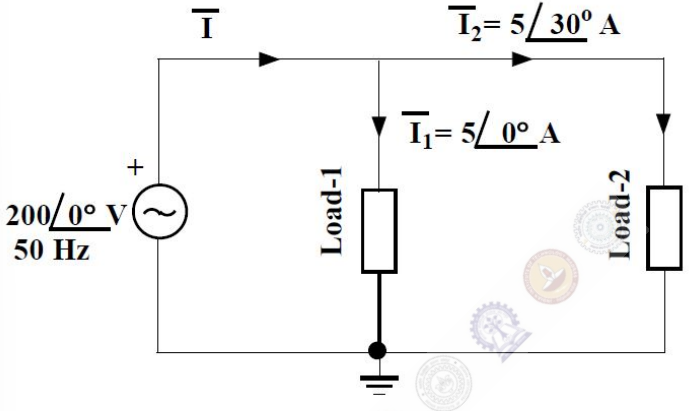
\includegraphics[width=0.5\textwidth]{figures/30.png}
\end{center}
\vspace{0.5cm}

\questionb{A series R-L-C circuit is excited with an a.c. voltage source. The quality factor (\(Q\)) of the circuit is given as \( Q = 30 \). The amplitude of current in \textbf{ampere} at upper half-power frequency will be \_\_\_\_\_.}{31}
\begin{center}
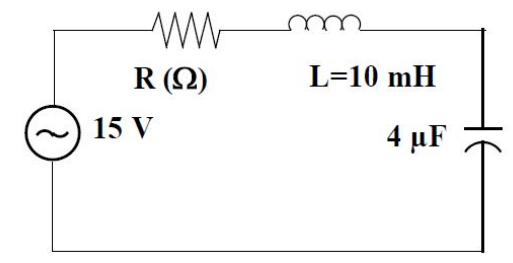
\includegraphics[width=0.5\textwidth]{figures/31.png}
\end{center}
\vspace{0.5cm}

\questionb{In the circuit diagram, shown in the figure, \( S_1 \) was closed and \( S_2 \) was open for a very long time. At \( t = 0 \), \( S_1 \) is opened and \( S_2 \) is closed. The voltage across the capacitor, in \textbf{volt}, at \( t = 5 \, \mu s \) is \_\_\_\_\_.}{32}
\begin{center}
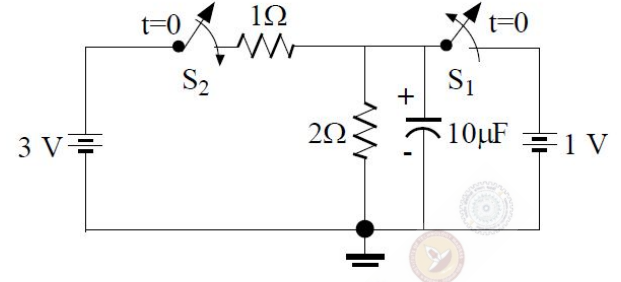
\includegraphics[width=0.5\textwidth]{figures/32.png}
\end{center}
\vspace{0.5cm}

\questionb{Consider two discrete-time signals:  
\( x_1(n) = \{1, 1\} \) and \( x_2(n) = \{1, 2\} \), for \( n = 0, 1 \).  

The Z-transform of the convoluted sequence \( x(n) = x_1(n) * x_2(n) \) is}{33}
\begin{enumerate}
    \item[(A)] \( 1 + 2z^{-1} + 3z^{-2} \)  
    \item[(B)] \( z^2 + 3z + 2 \)  
    \item[(C)] \( 1 + 3z^{-1} + 2z^{-2} \)  
    \item[(D)] \( z^{-2} + 3z^{-3} + 2z^{-4} \)
\end{enumerate}
\vspace{0.5cm}

\questionb{Three DFT coefficients, out of five DFT coefficients of a five-point real sequence are given as:  
\( X(0) = 4 \), \( X(1) = 1 - j1 \) and \( X(3) = 2 + j2 \). The zero-th value of the sequence \( x(n) \), \( x(0) \), is}{34}
\begin{enumerate}
    \item[(A)] 1  
    \item[(B)] 2  
    \item[(C)] 3  
    \item[(D)] 4  
\end{enumerate}
\vspace{0.5cm}

\questionb{The Laplace transform of a causal signal \( y(t) \) is  
\[ Y(s) = \frac{s+2}{s+6} \]  
The value of the signal \( y(t) \) at \( t = 0.1 \, s \) is \_\_\_\_\_ unit.}{35}
\vspace{0.5cm}

\questionb{The block diagram of a closed-loop control system is shown in the figure. The values of \( k \) and \( k_p \) are such that the system has a damping ratio of 0.8 and an undamped natural frequency \(\omega_n\) of 4 rad/s respectively. The value of \( k_p \) will be \_\_\_\_\_.}{36}
\begin{center}
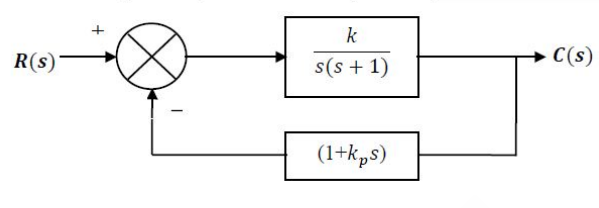
\includegraphics[width=0.5\textwidth]{figures/36.png}
\end{center}
\vspace{0.5cm}

\questionb{The loop transfer function of a closed-loop system is given by \( G(s)H(s) = \frac{K(s + 6)}{s(s + 2)} \). The breakaway point of the root-loci will be \_\_\_\_\_.}{37}
\vspace{0.5cm}

\questionb{A closed-loop system is shown in the figure. The system parameter \( \alpha \) is not known. The condition for asymptotic stability of the closed loop system is}{38}
\begin{center}
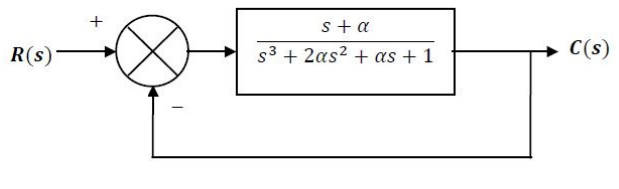
\includegraphics[width=0.5\textwidth]{figures/38.png}
\end{center}
\begin{enumerate}
    \item[(A)] \( \alpha < -0.5 \)  
    \item[(B)] \( -0.5 < \alpha < 0.5 \)  
    \item[(C)] \( 0 < \alpha < 0.5 \)  
    \item[(D)] \( \alpha > 0.5 \)
\end{enumerate}
\vspace{0.5cm}

\questionb{The overall closed loop transfer function \(\frac{c(s)}{R(s)}\), represented in the figure, will be}{39}
\begin{center}
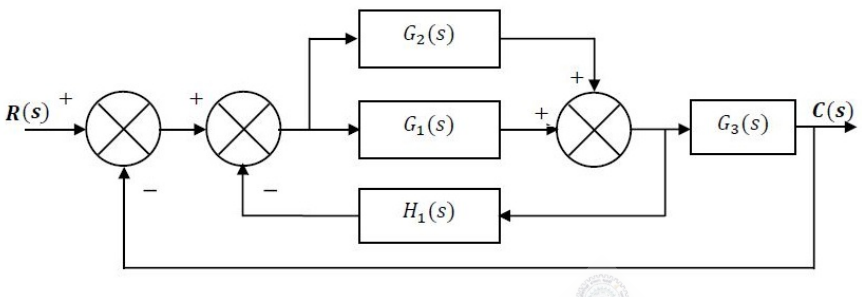
\includegraphics[width=0.8\textwidth]{figures/39.png}
\end{center}
\begin{enumerate}
    \item[(A)] \(\frac{(G_1(s)+G_2(s))G_3(s)}{1+(G_1(s)+G_2(s))(H_1(s)+G_3(s))}\)
    \item[(B)] \(\frac{(G_1(s)+G_3(s))}{1+G_1(s)H_1(s)+G_2(s)G_3(s)}\)
    \item[(C)] \(\frac{(G_1(s)-G_2(s))H_1(s)}{1+(G_1(s)+G_3(s))(H_1(s)+G_1(s))}\)
    \item[(D)] \(\frac{G_1(s)G_2(s)H_1(s)}{1+G_1(s)H_1(s)+G_1(s)G_3(s)}\)
\end{enumerate}
\vspace{0.5cm}

\questionb{Assuming the opamp shown in the figure to be ideal, the frequency at which the magnitude of \(V_0\) will be 95\% of the magnitude of \(V_{\text{in}}\) is \_\_\_\_\_ kHz.}{40}
\begin{center}
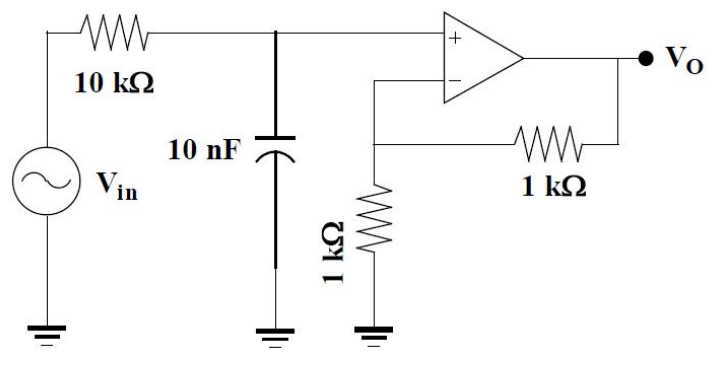
\includegraphics[width=0.5\textwidth]{figures/40.png}
\end{center}
\vspace{0.5cm}

\questionb{In the circuit, shown in the figure, the MOSFET is operating in the saturation zone. The characteristics of the MOSFET is given by \( I_D = \frac{1}{2} (V_{GS} - 1)^2 \) mA, where \( V_{GS} \) is in V. If \( V_S = +5 \, \text{V} \), then the value of \( R_S \) in kΩ is \_\_\_\_\_.}{41}
\begin{center}
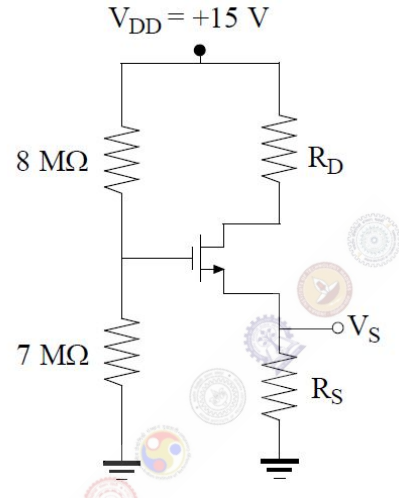
\includegraphics[width=0.5\textwidth]{figures/41.png}
\end{center}
\vspace{0.5cm}

\questionb{The two-input voltage multiplier, shown in the figure, has a scaling factor of 1 and produces voltage output. If \( V_1 = +15 \, \text{V} \) and \( V_2 = +3 \, \text{V} \), the value of \( V_0 \) in \textbf{volt} is \_\_\_\_\_.}{42}
\begin{center}
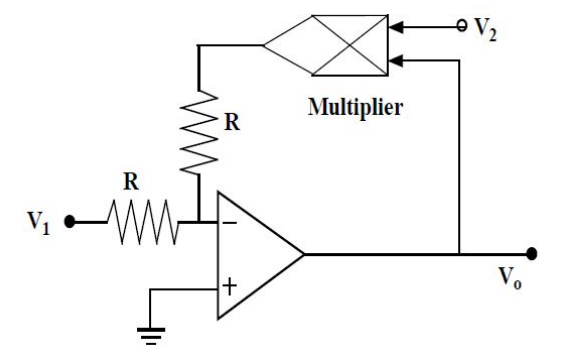
\includegraphics[width=0.5\textwidth]{figures/42.png}
\end{center}
\vspace{0.5cm}

\questionb{The two inputs A and B are connected to an R-S latch via two AND gates as shown in the figure. If \( A = 1 \) and \( B = 0 \), the output \( Q\overline{Q} \) is}{43}
\begin{center}
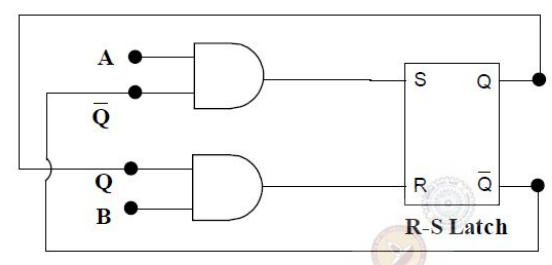
\includegraphics[width=0.5\textwidth]{figures/43.png}
\end{center}
\begin{enumerate}
    \item[(A)] 00  
    \item[(B)] 10  
    \item[(C)] 01  
    \item[(D)] 11
\end{enumerate}
\vspace{0.5cm}

\questionb{The circuit of a Schmitt trigger is shown in the figure. The zener-diode combination maintains the output between ± 7 V. The width of the hysteresis band is \_\_\_\_\_ V.}{44}
\begin{center}
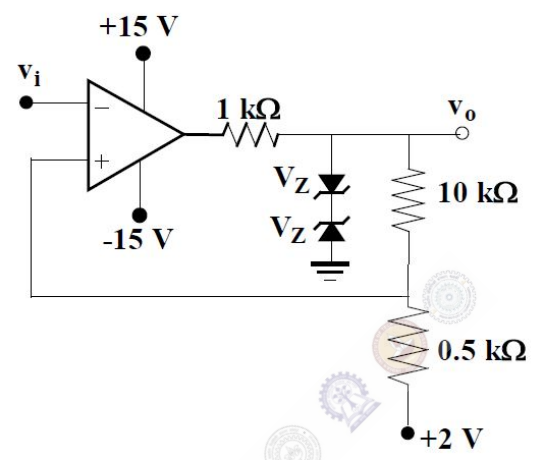
\includegraphics[width=0.5\textwidth]{figures/44.png}
\end{center}
\vspace{0.5cm}

\questionb{When the voltage across a battery is measured using a d.c. potentiometer, the reading shows 1.08 V. But when the same voltage is measured using a Permanent Magnet Moving Coil (PMMC) voltmeter, the voltmeter reading shows 0.99 V. If the resistance of the voltmeter is 1100 Ω, the internal resistance of the battery, in Ω, is \_\_\_\_\_.}{45}
\vspace{0.5cm}

\questionb{The power delivered to a single phase inductive load is measured with a dynamometer type wattmeter using a potential transformer (PT) of turns ratio 200:1 and the current transformer (CT) of turns ratio 1:5. Assume both the transformers to be ideal. The power factor of the load is 0.8. If the wattmeter reading is 200 W, then the apparent power of the load in kVA is \_\_\_\_\_.}{46}
\vspace{0.5cm}

\questionb{The unbalanced voltage of the Wheatstone bridge, shown in the figure, is measured using a digital voltmeter having infinite input impedance and a resolution of 0.1 mV. If \( R = 1000 \, \Omega \), then the minimum value of \(\Delta R\) in \(\Omega\) to create a detectable unbalanced voltage is \_\_\_\_\_.}{47}
\begin{center}
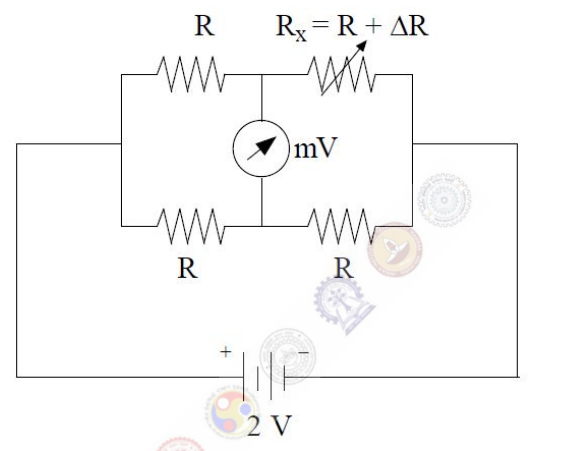
\includegraphics[width=0.5\textwidth]{figures/47.png}
\end{center}
\vspace{0.5cm}

\questionb{In the a.c. bridge, shown in the figure, \( R = 10^3 \, \Omega \) and \( C = 10^{-7} \, F \). If the bridge is balanced at a frequency \( \omega_0 \), the value of \( \omega_0 \) in rad/s is \_\_\_\_\_.}{48}
\begin{center}
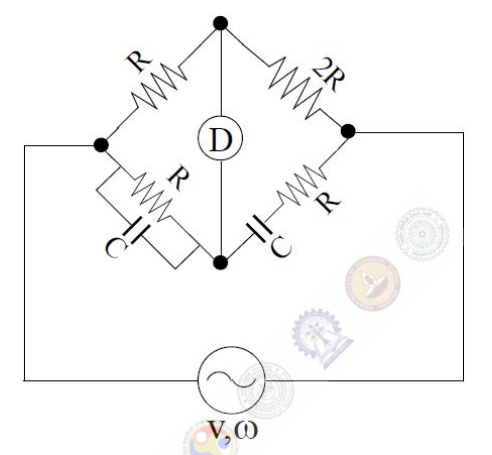
\includegraphics[width=0.5\textwidth]{figures/48.png}
\end{center}
\vspace{0.5cm}

\questionb{The hot junction of a bare thermocouple, initially at room temperature (30°C), is suddenly dipped in molten metal at \( t = 0 \, s \). The cold junction is kept at room temperature. The thermocouple can be modeled as a first-order instrument with a time constant of 1.0 s and a static sensitivity of 10 \(\mu V/^\circ C\). If the voltage, measured across the thermocouple indicates 10.0 mV at \( t = 1.0 \, s \), then the temperature of the molten metal in °C is \_\_\_\_\_.}{49}
\vspace{0.5cm}

\questionb{A resistance temperature detector (RTD) is connected to a circuit, as shown in the figure. Assume the opamp to be ideal. If \( V_o = +2.0 \, \text{V} \), then the value of \( x \) is \_\_\_\_\_.}{50}
\begin{center}
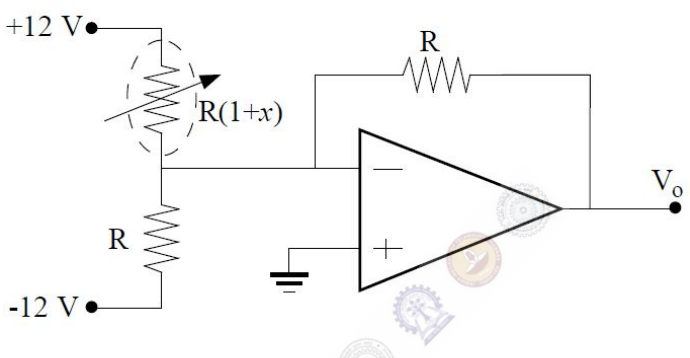
\includegraphics[width=0.5\textwidth]{figures/50.png}
\end{center}
\vspace{0.5cm}

\questionb{The magnetic flux density of an electromagnetic flowmeter is \( 100 \, \text{mWb/m}^2 \). The electrodes are wall-mounted inside the pipe having a diameter of \( 0.25 \, \text{m} \). A voltage of \( 1 \, \text{V} \) is generated when a conducting fluid is passed through the flowmeter. The volumetric flowrate of the fluid in \( \text{m}^3/\text{s} \) is \_\_\_\_\_.}{51}
\vspace{0.5cm}

\questionb{The junction semiconductor temperature sensor shown in the figure is used to measure the temperature of hot air. The output voltage \( V_O \) is 2.1 V. The current output of the sensor is given by I = T \(\mu\)A where T is the temperature in K. Assuming the opamp to be ideal, the temperature of the hot air in ℃ is approximately \_\_\_\_\_.}{52}
\begin{center}
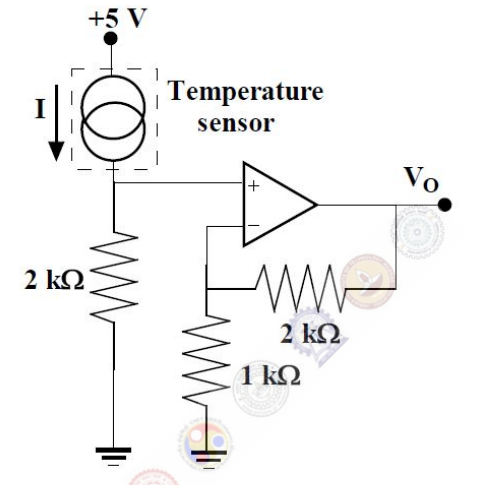
\includegraphics[width=0.5\textwidth]{figures/52.png}
\end{center}
\vspace{0.5cm}

\questionb{Quantum efficiency of a photodiode (ratio between the number of liberated electrons and the number of incident photons) is 0.75 at 830 nm. Given Planck's constant  
\( h = 6.624 \times 10^{-34} \, \text{J} \),  
the charge of an electron  
\( e = 1.6 \times 10^{-19} \, \text{C} \)  
and the velocity of light in the photodiode  
\( C_m = 2 \times 10^8 \, \text{m/s} \).  
For an incident optical power of 100 \(\mu\)W at 830 nm, the photocurrent in \(\mu\)A is \_\_\_\_\_.}{53}
\vspace{0.5cm}

\questionb{In a sinusoidal amplitude modulation scheme (with carrier) the modulated signal is given by  
\( A_m(t) = 100 \cos(\omega_c t) + 50 \cos(\omega_m t) \cos(\omega_c t) \),  
where \(\omega_c\) is the carrier frequency and \(\omega_m\) is the modulation frequency. The power carried by the sidebands in \% of total power is \_\_\_\_\_\%.}{54}
\vspace{0.5cm}

\questionb{An angle modulated signal with carrier frequency \(\omega_c = 2\pi \times 10^6 \, \text{rad/s}\) is given by  
\(\varphi_m(t) = \cos(\omega_c t + 5 \sin(1000\pi t) + 10 \sin(2000\pi t))\).  
The maximum deviation of the frequency in the angle modulated signal from that of the carrier is \_\_\_\_\_ \textbf{kHz}.}{55}
\vspace{0.5cm}

\vspace{5cm}
\begin{center}
\textbf{END OF THE QUESTION PAPER} \\
\rule{\textwidth}{0.5pt}
\end{center}

\end{document}
